Trabaje con la transformada unilateral $\mathcal L\{f\}(s)=\int_0^\infty e^{-st}f(t)\,dt$. Las funciones de entrada son causales. Use $H(t-a)=0$ para $t<a$ y $H(t-a)=1$ para $t\ge a$; sus valores aislados en saltos no alteran la transformada. Sea $f$ el pulso triangular con vértices $(0,0),(1,1),(2,0)$ y nulo fuera de $[0,2]$. Se dispone de
\[F(s)=\frac{(1-e^{-s})^2}{s^2}.\]
Las gráficas definen $g$ y $h$ (nulas después del último intervalo mostrado).
\begin{center}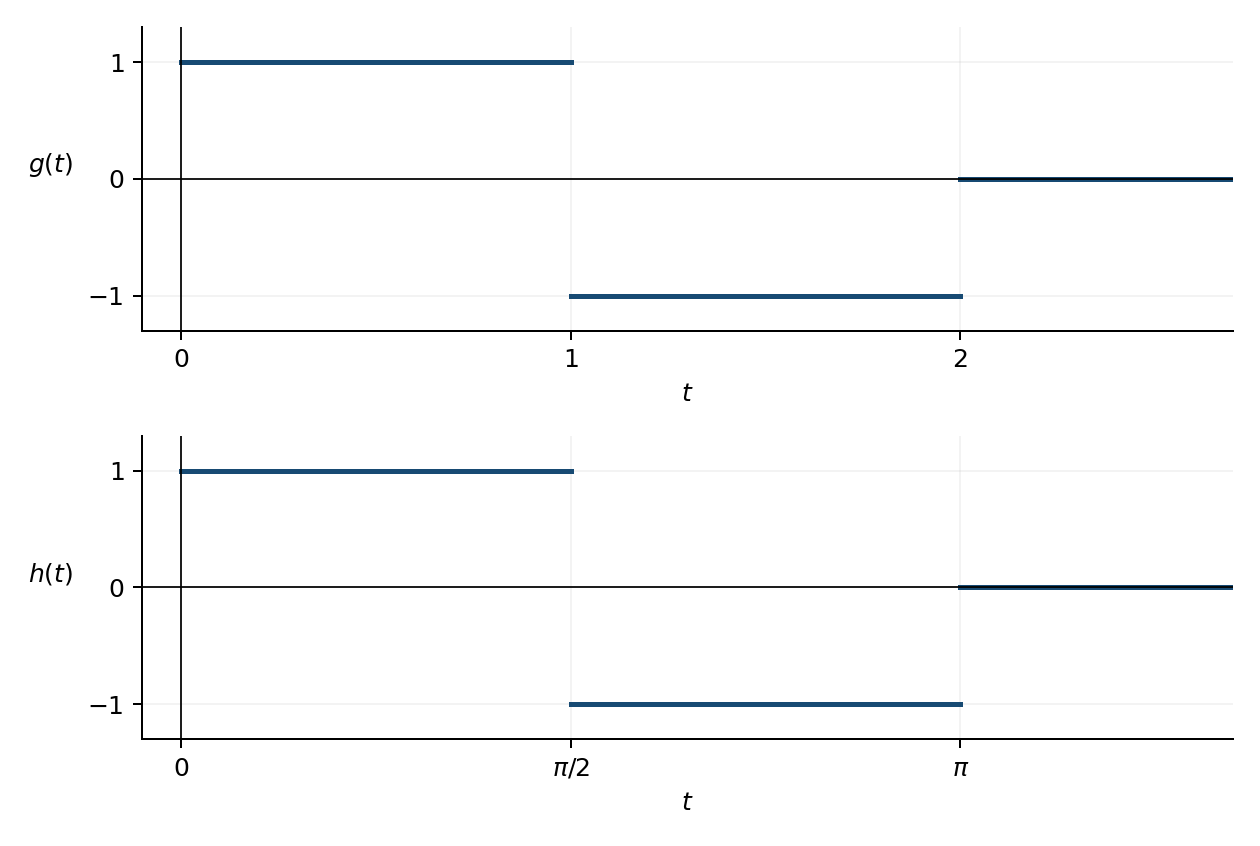
\includegraphics[width=.9\linewidth]{assets/M2-E0214-inputs.png}\end{center}

\begin{enumerate}[label=(\alph*),ref=\alph*,leftmargin=*]
\item Calcule la transformada de $g$, observando su relación con $f$.
\item Calcule la transformada de $h$, observando su relación con $g$.
\item Resuelva $y''+y=h(t)$, $y(0)=y'(0)=0$.
\end{enumerate}
